\section{Analyse paramétrique}
\paragraph{} Après avoir conçu l'outil de gestion du plant, il est intéressant d'analyser les résultats obtenus en
faisant varier les paramètres dans une plage réaliste. Les tableaux ci-dessous reprennent cette analyse. Nous avons
considéré une variation de température de \unit{800}{\kelvin} à \unit{1300}{\kelvin}. Ce choix a été déterminé par
les valeurs de référence utilisées dans le calcul de $K(T)$, qui sont pour la plupart valables jusqu'à
\unit{1300}{\kelvin}. En ce qui concerne la quantité d'ammoniac produite, nous avons testé de \unit{1000}{\ton \per jour} à
\unit{2000}{\ton \per jour}, étant donné que c'est la capacité typique d'un plant d'ammoniac.

\paragraph{} Le premier tableau fait varier la température, en considérant la quantité d'ammoniac \ce{NH_3} produite
par jour constante et valant \unit{1500}{\ton \per jour}.
\begin{table}[h!]
\centering
\begin{tabular}{|c||c|c|c|}
\hline
Température & Débit de méthane \ce{CH_4} & Débit de l'eau \ce{H_{2}O} & Débit d'air \\
\unit{\kelvin} & [\unit{\meter^3\per jour}] & [\unit{\meter^3\per jour}] & [\unit{\meter^3\per jour}] \\
\hline
800 & 86373.59 & 1044242.84 & 1.2518e+05 \\
\hline
900 & 97170.29 & 491179.16 & 1.4083e+05 \\
\hline
1000 & 107966.99 & 234055.84 & 1.5647e+05 \\
\hline
1100 & 118763.69 & 105168.26 & 1.7212e+05 \\
\hline
1200 & 129560.39 & 62398.32 & 1.8777e+05 \\
\hline
1300 & 140357.09 & 57193.98 & 2.0342e+05 \\
\hline
\end{tabular}
\caption{La température $T$ varie, la quantité d'ammoniac \ce{NH_3} produite par jour est constante}
\label{tab:tvarie}
\end{table}
\paragraph{} Le deuxième tableau fait varier la quantité d'ammoniac \ce{NH_3}, en considérant la température $T$ constante et
valant \unit{1000}{\kelvin}.
\begin{table}[h!]
\centering
\begin{tabular}{|c||c|c|c|}
\hline
Production journalière de \ce{NH_3} & Débit de méthane \ce{CH_4} & Débit de l'eau \ce{H_{2}O} & Débit d'air \\
\unit{\ton \per jour} & [\unit{\meter^3\per jour}] & [\unit{\meter^3\per jour}] & [\unit{\meter^3\per jour}] \\
\hline
\hline
1000 & 71978.00 & 156037.22 & 1.0432e+05 \\
\hline
1100 & 79175.80 & 171640.95 & 1.1475e+05 \\
\hline
1200 & 86373.59 & 187244.67 & 1.2518e+05 \\
\hline
1300 & 93571.39 & 202848.39 & 1.3561e+05 \\
\hline
1400 & 100769.19 & 218452.11 & 1.4604e+05 \\
\hline
1500 & 107966.99 & 234055.84 & 1.5647e+05 \\
\hline
1600 & 115164.79 & 249659.56 & 1.6691e+05 \\
\hline
1700 & 122362.59 & 265263.28 & 1.7734e+05 \\
\hline
1800 & 129560.39 & 280867.00 & 1.8777e+05 \\
\hline
1900 & 136758.19 & 296470.73 & 1.9820e+05 \\
\hline
2000 & 143955.99 & 312074.45 & 2.0863e+05 \\
\hline
\end{tabular}
\caption{La quantité d'ammoniac \ce{NH_3} produite par jour varie, la température $T$ est constante}
\label{tab:nh3varie}
\end{table}

\newpage
Nous devions surtout surveiller la quantité d'eau, étant donné qu'elle devait être en excès dans les réactions à
l'équilibre, pour qu'il reste assez de vapeur afin de permettre une conversion complète de \ce{CO} en \ce{CO2} dans le
réacteur Water-Gas-Shift.
Nous avons donc déterminé la température critique à partir de laquelle la quantité d'eau sortante devenait nulle.
Nous sommes arrivés à la conclusion qu'il faut limiter la température de sortie du reformeur primaire à
\unit{1049.472}{\kelvin}, si nous voulons une capacité d'ammoniac de \unit{1500}{\ton\per jour}.
Le graphe suivant permet de visualiser ce qui sort vraiment de notre installation. Les valeurs ont été calculées pour
avoir 1500t d'ammoniac au final. Il est donc normal de constater que l'ammoniac apparaît en ligne droite.
Nous pouvons égalemnt bien visualiser qu'à partir de la température de \unit{1050}{\kelvin}, le débit d'eau sortant devient
négatif; chose problématique comme expliqué ci-dessus.
Le \ce{CO2} et l'argon sortant sont quant à eux constants en fonction de la température. L'argon est rejeté en petites quatités, mais le \ce{CO2}
apparaît en quantités plus importantes malheureusement.
\begin{figure}[ht!]
\centering
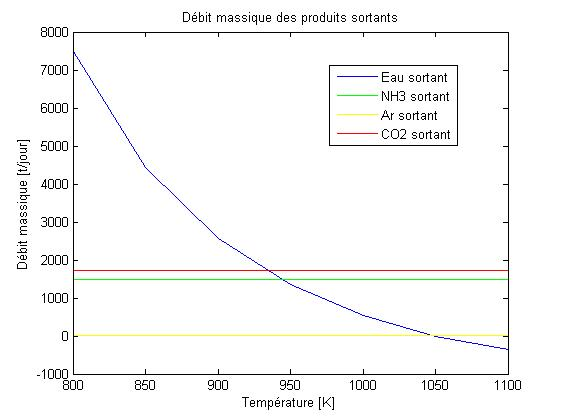
\includegraphics[scale=0.6]{produits.jpg}
\label{produits_sortants}
\end{figure}
